\documentclass[twocolumn]{aastex631}

\shorttitle{Earth Migration and Mars Encounters}
\shortauthors{Laughlin}

\begin{document}

\title{Close Earth--Mars Encounters in a Numerical Experiment that Moves Earth Outward}

\author{Gregory Laughlin}
\affiliation{Department of Astronomy, Yale University, New Haven, CT, USA}

\begin{abstract}
We describe a numerical stress test inspired by the long-term planetary-engineering scenario of \citet{korycansky2001}.  Rather than model repeated asteroid-mediated gravity assists, we apply direct impulsive velocity increments to Earth in the direction of its instantaneous heliocentric motion.  The impulses are timed at random orbital phases and normalized so that a two-body energy estimate would move Earth from approximately 1 AU to 1.4 AU over 10 Myr.  In five representative REBOUND integrations with 2000 impulses, Earth reaches final semimajor axes between 1.374 and 1.444 AU, while Mars undergoes large secular and resonant responses, ending with semimajor axes from 1.208 to 2.692 AU.  Follow-up encounter searches using a 50,000 km Earth--Mars screening distance and IAS15 refinement identified a non-collisional near miss with center-to-center separation 16,512 km, corresponding to a surface clearance of 6,752 km, or 1.69 summed planetary radii.  The experiments are not a feasible engineering prescription and do not constitute a statistical collision probability calculation.  They demonstrate, however, that outward migration of Earth by direct prograde energy injection can strongly perturb Mars and can generate encounters in the regime where tidal and geophysical consequences would be severe.
\end{abstract}

\keywords{Celestial mechanics (211) --- Solar System dynamics (2001) --- Planetary dynamics (2173) --- N-body simulations (1083)}

\section{Introduction}

\citet{korycansky2001} proposed that planetary orbits could in principle be engineered over gigayear timescales by using repeated asteroid or comet encounters to transfer orbital energy and angular momentum.  That mechanism was designed to avoid applying rocket-like impulses directly to Earth, and to recycle energy through resonant encounters involving Jupiter and smaller bodies.  The present calculation is intentionally different.  It asks what happens in a deliberately simplified Solar System experiment where Earth is pushed directly and repeatedly in the prograde direction.

The calculation is therefore best viewed as a dynamical stress test.  It is useful for visualization and for developing intuition about how strongly the terrestrial planets can respond when Earth's orbit is moved through the inner Solar System architecture.  It is not a mission design, and it omits the intermediate bodies and control logic that would be required in any physically motivated version of the original proposal.

\section{Numerical Setup}

All integrations use the Sun, the eight planets, and Pluto initialized from the JPL DE440s ephemeris at 2026 July 22, 14:00 UTC, corresponding to 9:00 a.m. Central Daylight Time.  The simulations use astronomical units, solar masses, and Julian years.  The main integrations use REBOUND \citep{rebound} with the WHFast symplectic integrator \citep{whfast}, an 8 day timestep, Jacobi coordinates, and an 11th-order symplectic corrector.

For the fiducial kicked-Earth experiment, impulses are applied directly to Earth at random times over a 10 Myr kick interval.  Each impulse is parallel to Earth's instantaneous velocity.  The kick normalization is set by the two-body specific orbital energy difference between an initial circular orbit at $a_0 \simeq 1\,{\rm AU}$ and a target orbit at $a_f = 1.4\,{\rm AU}$,
\begin{equation}
    \Delta \epsilon =
    {GM_\odot \over 2}\left({1 \over a_0} - {1 \over a_f}\right).
\end{equation}
For $N_{\rm kick}=2000$ impulses, each event receives $\Delta \epsilon_i = \Delta \epsilon/N_{\rm kick}$.  If $v_t$ is the instantaneous tangential speed, the applied increment is
\begin{equation}
    \Delta v_i = -v_t + \left(v_t^2 + 2\Delta\epsilon_i\right)^{1/2}.
\end{equation}
For the default initial state this gives a cumulative applied impulse of 4.61 km s$^{-1}$.  The random seed fixes both the kick times and phases, making each run exactly reproducible within a fixed software environment.

Earth--Mars close approaches are first detected using REBOUND's line collision machinery configured with a non-destructive callback.  In the search runs, the line-collision radius is a screening threshold rather than a physical impact radius.  Candidate events are then replayed and refined by switching to IAS15 \citep{ias15} over a local time window and minimizing the Earth--Mars separation.  We quote refined encounter distances only for candidates that survive this replay.

\section{Results}

\subsection{Five-seed 10 Myr sweep}

The initial animation campaign used seeds 20260722--20260726, 2000 impulses, and a 10 Myr integration.  Across these five examples, Earth's final semimajor axis lies between 1.374 and 1.444 AU.  The range is close to the two-body target, but the resulting eccentricities and the angular relation to Mars differ from seed to seed.

Mars responds more dramatically.  In the same five runs, Mars' final semimajor axis ranges from 1.208 to 2.692 AU, and its final eccentricity reaches 0.443.  The closest approach in this first sweep occurs for seed 20260725 at $t=9.227$ Myr, with center-to-center separation $0.001069$ AU.  This is approximately $1.60\times 10^5$ km, or 16.4 times the sum of the Earth and Mars radii, and is not a collision.  Figure~\ref{fig:seed-sweep} shows the semimajor-axis evolution for the five runs.

\begin{figure*}
\centering
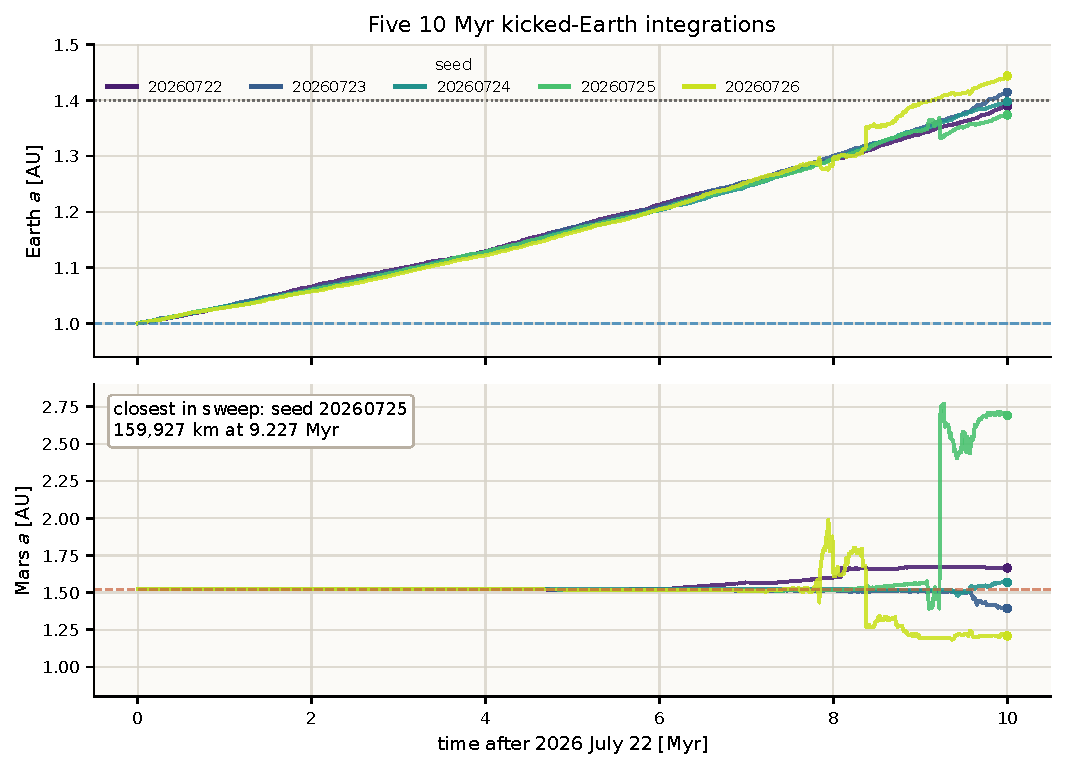
\includegraphics[width=0.92\textwidth]{figures/move_earth_seed_sweep_semimajor_axes.pdf}
\caption{
Semimajor-axis evolution in the five 10 Myr kicked-Earth integrations used for the initial animation sweep.  Each colored curve is a different random seed.  Earth is driven outward toward the two-body target near 1.4 AU, while Mars shows a much larger seed-dependent response.  The dashed horizontal lines mark the initial Earth and Mars semimajor axes, and the dotted line marks the nominal 1.4 AU Earth target.
}
\label{fig:seed-sweep}
\end{figure*}

\subsection{Refined close-encounter search}

After the initial sweep, the search was restarted on fresh seeds with a 50,000 km Earth--Mars screening threshold.  Some integrations extended the kick period and then continued without further impulses so that the perturbed planetary system could evolve.  The closest refined case found so far is seed 20260917.  The refined minimum occurs at
\begin{equation}
    t = 9.210348154884227\,{\rm Myr}
\end{equation}
after the initial epoch, with Earth--Mars center-to-center distance 16,512 km.  Taking $R_\oplus + R_{\rm Mars}=9760.5$ km, the surface clearance is 6,752 km, or 1.69 summed radii.  The bodies do not physically collide in the refined integration.

A second notable close encounter is seed 20260906.  Its refined minimum distance is 36,516 km center-to-center, corresponding to a surface clearance of 26,755 km, or 3.74 summed radii.  This case is useful as a less extreme but still visually dramatic non-collisional encounter.

\begin{figure*}
\centering
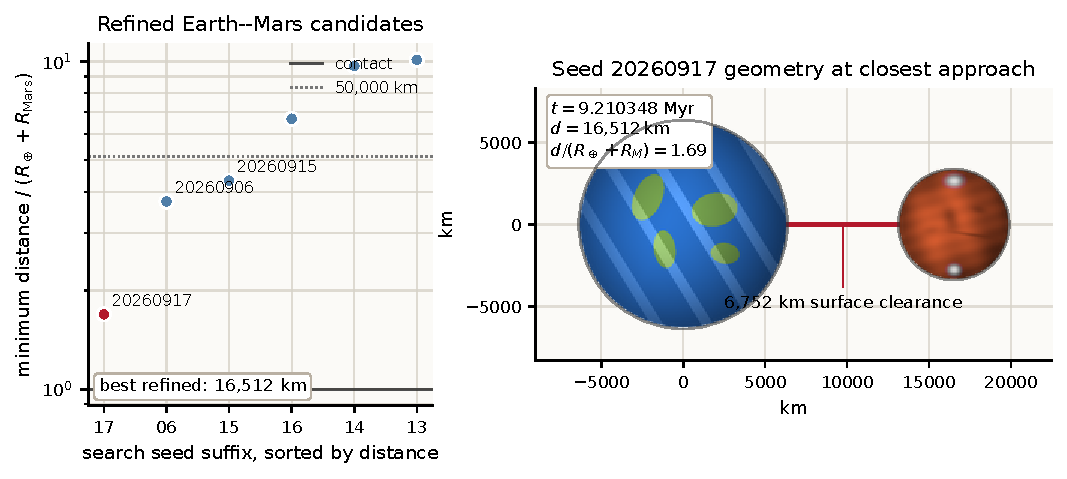
\includegraphics[width=0.92\textwidth]{figures/move_earth_refined_encounters.pdf}
\caption{
Refined close-encounter candidates and the geometry of the closest event found so far.  Left: candidate Earth--Mars minimum distances after IAS15 replay/refinement, plotted in units of $R_\oplus+R_{\rm Mars}$.  The solid horizontal line is physical contact, and the dotted line is the 50,000 km screening threshold.  Right: a true-scale view of the seed 20260917 encounter at the refined minimum.  The Earth and Mars image textures are the same procedural visual assets used in the animation workflow, redrawn here on a light publication background.
}
\label{fig:refined-encounters}
\end{figure*}

\section{Discussion}

The simulations show that a direct prograde energy-injection rule can move Earth outward on the intended order of magnitude, but the resulting evolution is not isolated to Earth.  Mars is readily driven into large changes in semimajor axis and eccentricity.  The sensitivity to seed indicates that the phasing of impulses relative to the terrestrial planets, and to the resonant structure traversed by Earth and Mars, matters as much as the scalar energy budget.

The closest refined encounter found to date, with 6,752 km surface clearance, is well inside the regime where the event would be catastrophic for both planets.  Such a passage would involve severe tides, strong deformation of the oceans and solid bodies, intense seismic and volcanic excitation, and major changes to the orbits and spins.  The experiment does not by itself compute the hydrodynamic or geophysical response; that would require a separate close-encounter calculation with appropriate planetary interior and surface models.  The N-body result supplies a plausible encounter geometry for such follow-up simulations.

The line-collision logs should not be interpreted as exact continuous closest-approach measurements.  They are an efficient way to identify candidate intervals.  One threshold-triggered candidate in the campaign did not reproduce as a close encounter under refined replay, underscoring the need to quote only refined distances for physical interpretation.

\section{Limitations}

The calculations omit general relativity, asteroid belts, mass loss, tides, oblateness, and any feedback control of the impulses.  The direct kicks violate the spirit of the gravity-assist scheme of Korycansky et al. because they inject energy into Earth locally rather than exchanging it through smaller bodies.  The seed search is also intentionally biased toward finding dramatic Earth--Mars encounters, so the current set of runs cannot be used to infer an encounter rate or impact probability.

\section{Conclusions}

Directly pushing Earth outward with many small prograde impulses is dynamically hazardous in these integrations.  A 10 Myr, 2000-kick experiment can place Earth near the intended 1.4 AU scale, but Mars can be strongly destabilized.  Refined searches have found non-collisional Earth--Mars passages as close as 16,512 km center-to-center, only 6,752 km above nominal surface contact.  These runs provide a useful numerical and visual demonstration that any planetary migration scheme must control not only Earth's energy but also the angular-momentum exchange and resonant response of the rest of the terrestrial system.

\section{Software and Data Availability}

The scripts used to generate the integrations, close-encounter searches, refined replays, and animation products are available in the public repository \texttt{oklo/solar\_system\_integration}.  Large generated movies, raw close-encounter logs, and long output directories are intentionally excluded from version control.

\begin{thebibliography}{99}

\bibitem[Korycansky et al.(2001)]{korycansky2001}
Korycansky, D. G., Laughlin, G., \& Adams, F. C. 2001, \apss, 275, 349, doi:10.1023/A:1002790227314

\bibitem[Rein \& Liu(2012)]{rebound}
Rein, H., \& Liu, S.-F. 2012, \aap, 537, A128, doi:10.1051/0004-6361/201118085

\bibitem[Rein \& Tamayo(2015)]{whfast}
Rein, H., \& Tamayo, D. 2015, \mnras, 452, 376, doi:10.1093/mnras/stv1257

\bibitem[Rein \& Spiegel(2015)]{ias15}
Rein, H., \& Spiegel, D. S. 2015, \mnras, 446, 1424, doi:10.1093/mnras/stu2164

\end{thebibliography}

\end{document}
